\documentclass{article}

\usepackage{Mathematics}
\makeatletter
\@fleqnfalse
\makeatother

\pdftitle{SW5-Math1A-tutoring}

% === TITLE ===
\title{\textbf{Mathematics 1A Tutoring session\\ Semester Week 5}}
\author{Matteo Frongillo}
\date{}

\newcommand{\exercise}[2][]{%
  \par\noindent\textbf{Exercise \thesection.#1:\\} #2\par \vspace*{.25cm}
}

\newcommand{\solution}[2][]{%
  \par\noindent\textbf{Solution #1:\\} #2\par \vspace*{.25cm}
}

% === TEXT ===
\begin{document}

\maketitle

\part*{Exercises}
\section{Trigonometry}
\exercise[1]{
  Find the hypotenuse of a right triangle with adjacend side $b = 36.4$ cm and opposite side $c = 41.8$ cm.
}

\exercise[2]{
  Solve a right triangle where only the hypothenuse $a=3$ cm and the angle $\beta = 34,7^\circ$ are known.
}

\exercise[3]{
  Determine domain and range of the following trigonometric functions:
  \begin{center}
    \[
      \sin\left(x\right)\quad ; \quad
      \cos^{-1}\left(x\right)\quad ; \quad
      \tan\left(x\right)\quad ; \quad
      \arctan\left(x\right)
    \]
  \end{center}
}

\exercise[4]{
  A block of mass $m = 2\,\mathrm{kg}$ rests on an inclined plane that forms an angle $\theta$ with the horizontal.
  The gravitational acceleration is $g = 9.81\,\mathrm{m\,s^{-2}}$.
  \begin{enumerate}[label=\alph*.]
    \item Express the components of the force parallel and perpendicular to the plane, $F_\parallel$ and $F_\perp$, as functions of $\theta$, knowing that $F = m g$.
    \item Compute $F_\parallel$ and $F_\perp$ for $\theta = 25^\circ$.
    \item Find the value of $\theta$ for which $F_\parallel = \dfrac{1}{2} F_\perp$.
    \item Determine the length $L$ of the inclined plane knowing that the height is $h = 1.5\,\mathrm{m}$ and the horizontal projection is $x = 3.3\,\mathrm{m}$.
  \end{enumerate}
}

\exercise[5 {\color{red}BONUS}]{\\
  \begin{minipage}{0.3\textwidth}
    \begin{center}
      \includegraphics[width=.8\textwidth]{media/trig_sw5.png}
    \end{center}
  \end{minipage}
  \hfill
  \begin{minipage}{0.65\textwidth}
    A cube $ABCDEFGH$ with edge length 8 cm is given.\\
    Point $M$ is defined so that $\overrightarrow{EM} = \dfrac{2}{5}\,\overrightarrow{EG}$.\\
    Calculate the measure of the sides and angles of triangle $ACM$
  \end{minipage}
}

\newpage
\section{Exponential functions}
\exercise[1]{
  Determine the half-life of a radioactive substance $X$, knowing that after
  one year its mass has decreased to one third.
}

\exercise[2]{
  A sample of St-89 (Strontium-89, a radioactive element with $T=50.5$ days)
  has lost 2 g of mass after one month.
  Determine the mass of the same initial sample after one year.

  Hint: for decays, $k = -\dfrac{\ln(2)}{T}$
}

\exercise[3]{
  Solve in $\mathbb{R}$ \textbf{without the calculator}:
  \[
    \log\left(x^2\right) = 3\quad ; \quad
    \ln\left(x+1\right)=\frac{1}{2}\quad ; \quad
    \ln\left(x+1\right)=0.001^2\quad ; \quad
    \log_2\left(x^2-4x+4\right)=2\quad ; \quad
    \left(x^2+x-2\right)\ln(2x)=0
  \]
}

\exercise[4]{
  A hot object with an initial temperature $T_0$, placed at time $t=0$ in an environment with lower temperature $T_1$, cools according to Newton's law of cooling:
  \figbox{$T=T_1 + \left(T_0 - T_1\right) e^{-kt}$}\\
  where $T$ is the temperature of the object at time $t$, and $k$ is a constant depending on the material of the object.

  Consider a steel sphere heated to $133^\circ$C and then placed to cool in a room where the air temperature is $22^\circ$C.\\
  Calculate:
  \begin{enumerate}[label=\alph*.]
    \item the temperature of the sphere after 20 minutes, knowing that after 10 minutes it had cooled to $108^\circ$C;
    \item the time required for the temperature to drop to $66.5^\circ$C.
  \end{enumerate}
}

\section{Composite functions}
\exercise[1]{
  Let $f: \mathbb{R} \to \mathbb{R}$

  \[x \mapsto y =
    \begin{cases}
      \dfrac{1}{2}x+1\ , &\text{for } x \geq 4\\
      x-1\ , &\text{for } -1 < x < 4\\
      -2x-4\ , &\text{for } x\leq -1
    \end{cases}
  \]

  Solve:
  \noindent
  \begin{minipage}[t]{0.3\textwidth}
    \begin{enumerate}[label=\alph*.,itemsep=1em]
      \item $f(0)$
      \item $f(-11)$
    \end{enumerate}
  \end{minipage}%
  \hfill
  \begin{minipage}[t]{0.3\textwidth}
    \begin{enumerate}[label=\alph*.,resume,itemsep=1em]
      \item $f\!\left(\tfrac{9}{2}\right)$
      \item $f\!\left(f\!\left(-\tfrac{1}{2}\right)\right)$
    \end{enumerate}
  \end{minipage}%
  \hfill
  \begin{minipage}[t]{0.3\textwidth}
    \begin{enumerate}[label=\alph*.,resume,itemsep=1em]
      \item $f(6)-f(-6)$
      \item $f\!\left(3f(-1)-2f(2)\right)$
    \end{enumerate}
  \end{minipage}
}

\exercise[2]{
  Let $f: \mathbb{R} \to \mathbb{R}$

  \[x \mapsto y =
    \begin{cases}
      \dfrac{1}{2}x\ , &\text{for } x < -2\\[2.5ex]
      \dfrac{2}{3}x + 1\ , &\text{for } -2 \leq x \leq 2\\[2.5ex]
      \dfrac{x+2}{3}\ , &\text{for } x > 2
    \end{cases}
  \]

  Solve:
  \[
    a.\ f\left(\frac{6}{5}\right)\quad ; \quad
    b.\ f\big(f\left(-3\right)\big)\quad ; \quad
    c.\ 2\big(f\left(7\right)-1\big)^2
  \]
}

\section{Limits}
\exercise[1]{
  Solve the following limits using the dominant term method:
  \begin{gather*} \dm
    \lim_{x\to\infty} \frac{\left(x+1\right)^2}{x^2+1}\quad ; \quad \lim_{x\to\infty} \frac{\sin(x)}{x}\quad ; \quad \lim_{x\to\infty} \frac{1000x}{x^2+1}\quad ; \quad \lim_{x\to\infty} \frac{x^2-5x+1}{3x+7}\\[2.5ex]
    \lim_{x\to\infty} \frac{2x^2-x+3}{x^3-8x+5}\quad ; \quad \lim_{x\to\infty} \frac{\left(2x+3\right)^3\left(3x-2\right)^2}{x^5+5}\quad ; \quad \lim_{x\to\infty} \frac{2x^2-3x-4}{\sqrt[3]{x^4+1}}
  \end{gather*}
}

\exercise[2]{
  For each of the following, determine whether the statement is true or false:
  \begin{center}
    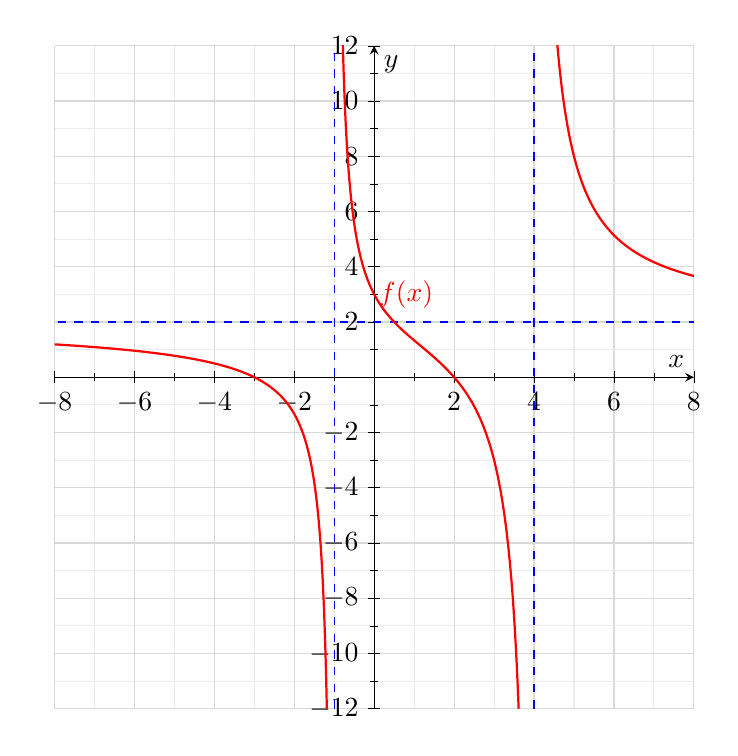
\begin{tikzpicture}
      \begin{axis}[
        axis lines=middle,
        width=.8\textwidth, height=10cm,
        xmin=-8, xmax=8,
        ymin=-12, ymax=12,
        xtick={-10,-8,...,10},
        ytick={-12,-10,...,12},
        grid=both,
        major grid style={gray!30},
        minor grid style={gray!15},
        minor tick num=1,
        tick style={black},
        xlabel={$x$},
        ylabel={$y$},
        restrict y to domain=-15:15,
        unbounded coords=jump,
        clip=true
      ]

      \addplot[dashed, blue] coordinates {(-10,2) (10,2)};
      \addplot[dashed, blue] coordinates {(-1,-15) (-1,15)};
      \addplot[dashed, blue] coordinates {(4,-15) (4,15)};

      \addplot[thick, red, samples=1500, domain=-10:10]
        {2+(8*x - 4)/((x + 1)*(x - 4))};

      \node[red] at (.8,3) {$f(x)$};
      \end{axis}
    \end{tikzpicture}
  \end{center}

  \begin{gather*}
    \text{a}) \lim_{x\to\infty} f(x)=0\quad , \quad \text{b}) \lim_{x\to 0} f(x)=2\quad , \quad \text{c}) \lim_{x\to 4^-} f(x) = +\infty\quad , \quad \text{d}) \lim_{x\to-1} f(x)=f(-1)\\[2ex]
    \text{e}) \lim_{x\to0} f(x) = 3\quad , \quad \text{f}) \lim_{x\to\infty} f(x)=-1\quad , \quad \text{g})\ f(x)=0 \iff x \in \left\{-3,4\right\}
  \end{gather*}
}

\exercise[3 (From Question 4.1, Homeworks Week 4)]{
  Are the following claims true or false? Explain why:
  \begin{enumerate}[label=\alph*.]
    \item If a function $y$ of $x$ is not defined at the position $x=x_0$, then $\dm \lim_{x\to x_0}$ does not exist either
    \item If $\dm \lim_{x\to x_0}$ does not exist, then $y$ is also not defined at the point $x=x_0$
    \item If a function $y$ of $x$ is defined at the position $x=x_0$, then $\dm \lim_{x\to x_0} y = y \big|_{x=x_0}$
    \item If $x$ approaches $1.000.000$ from the left, $1/x$ gets closer to the value 0. Therefore, $\dm \lim_{x \to 1.000.000^-} \frac{1}{x}=0$
    \item If $y$ has limit value 5 when $x$ approaches 3 from the left, then $y$ must already assume the value 5 in the range $x<3$
  \end{enumerate}
}



\newpage
\part*{Quick solutions}
\solution[1.1]{
  a = 55.43 cm
}

\solution[1.2]{
  b = 1.71 cm, c = 2.47 cm, $\alpha$ = 55.3$^\circ$
}

\solution[1.3]{\vspace*{-.5cm}
  \begin{enumerate}
    \item $\mathcal{D}_f = \forall x \in \mathbb{R}, \quad Im_f = \left[-1,1\right]$
    \item $\mathcal{D}_f = \left[-1,1\right], \quad Im_f = \left[\pi, 0\right]$
    \item $\mathcal{D}_f = \forall x \in \mathbb{R} \ \left\{\dfrac{\pi}{2}+k\pi \sht k \in \mathbb{Z}\right\}, \quad Im_f = \left[-1,1\right]$
    \item $\mathcal{D}_f = \forall x \in \mathbb{R}, \quad Im_f = \left[-\dfrac{\pi}{2}, \dfrac{\pi}{2}\right]$
  \end{enumerate}
}

\solution[1.4]{
  \vspace*{-0.5cm}
  \begin{enumerate}[label=\alph*.]
    \item $F_\parallel = mg\cos(x)\ , \quad F_\perp = mg\sin(x)$
    \item $F_\parallel = 17.78$ N, $\quad F_\perp = 8.29$ N
    \item $\theta = 0.46 \text{ rad} = 26.6^\circ$
    \item $L = 3.6$ m
  \end{enumerate}
}

\solution[1.5]{
  $\overrightarrow{AC} = 8\sqrt(2)$ cm $\approx 11.3$ cm\\[2ex]
  $\overrightarrow{AM} = \dfrac{8\sqrt(33)}{5}$ cm $\approx 9.19$ cm\\[2ex]
  $\overrightarrow{MC} = \dfrac{8\sqrt(43)}{5}$ cm $\approx 10.49$ cm\\[2ex]
  $\widehat{MAC}: \alpha \approx 60.5^\circ $\\[2ex]
  $\widehat{ACM}: \beta \approx 49.7^\circ$\\[2ex]
  $\widehat{AMC}: \gamma \approx 69.8^\circ$
}

\solution[2.1]{
  Half-time: 0.63 years $\approx$ 230 days
}

\solution[2.2]{
  $m_0 = 5.93$ g
}

\solution[2.3]{
  \begin{enumerate}[label=\alph*.]
    \item $\dm x = \pm \sqrt{10^3}$
    \item $\dm x = e^{\tfrac{1}{2}}-1$
    \item $\dm x = e^{10^{-6}}-1 \approx 0$
    \item $\dm x_1 = 0,\ x_2 = 4$
    \item $\dm x \in \left\{-2, \dfrac{1}{2}, 1\right\}$
  \end{enumerate}
}

\solution[2.4]{
  \begin{enumerate}[label=\alph*.]
    \item $T = 88.63^\circ$C
    \item $t \approx 35.2$ min
  \end{enumerate}
}

\solution[3.1]{
  \begin{enumerate}[label=\alph*.]
    \item $f(0) = 1$
    \item $f(-11)=18$
    \item $f\left(\dfrac{9}{2}\right) = \dfrac{13}{4}$
    \item $f\left(f\left(-\dfrac{1}{2}\right)\right) = -1$
    \item $f(6) - f(-6) = -4$
    \item $f\big(3f(-1)-2f(2)\big) = 12$
  \end{enumerate}
}

\solution[3.2]{
  \begin{enumerate}[label=\alph*.]
    \item $f\left(\dfrac{6}{5}\right) = \dfrac{9}{5}$
    \item $f\big(f(-3)\big) = 0$
    \item $2\big(f(7)-1\big)^2=8$
  \end{enumerate}
}

\solution[4.1]{
  \begin{enumerate}[label=\alph*.]
    \item = 1
    \item = 0
    \item = 0
    \item = 0
    \item = 72
    \item = $\infty$
  \end{enumerate}
}

\solution[4.2]{
  \begin{enumerate}[label=\alph*.]
    \item False
    \item False
    \item False
    \item False
    \item True
    \item False
    \item False
  \end{enumerate}
}

\solution[4.3]{
  All the statements are False
}

\end{document}
